Após a construção da ISS, surgiu a necessidade de realizar a atracação (\emph{berthing}) para que os módulos espaciaios de carga como a espaçonave \emph{Cygnus} dos Estados Unidos da América e o veículo não-tripulado japonês HTV (\emph{H-II Transfer Vehicle}) pudessem se conectar na estação espacial através do manipulador robótico Canadarm2.

\section{Cygnus}

A atracação da espaçonave \emph{Cygnus} à ISS representa um marco na colaboração entre agências espaciais e empresas privadas para o avanço das operações em órbita baixa.
A \emph{Cygnus} é um veículo de reabastecimento não-tripulado e foi desenvolvida pela \emph{Northrop Grumman} para transportar cargas como suprimentos, equipamentos e experimentos científicos para a ISS.
Durante essas missões, a \emph{Cygnus} se aproximava da estação e era capturada pelo manipulador robótico \emph{Canadarm2}, que era operada pelos astronautas a bordo da ISS, portanto eles finalizavam o processo de atracação, conectando a espaçonave a um dos módulos de atração da ISS \cite{nasaCygnus}.

\begin{figure}[ht]
    \centering
    \includegraphics[width=1\linewidth]{1 Introducao/Imagens/Cygnus Northrop Grumman.png}
    \caption{Espaçonave cargueira Cygnus e o Canadaarm2. Fonte: NASA.}
    \label{fig:CygnusFoto}
\end{figure}

A capacidade da Cygnus de regularmente realizar missões de reabastecimento destaca a importância de parcerias público--privadas no suporte contínuo às operações da ISS.
Essas missões não só permitem o fornecimento de recursos fundamentais, mas também reforçam a infraestrutura para condução de pesquisas científicas ambiente de microgravidade.
O sucesso dessas missões de reabastecimento demonstra a maturidade e a confiabilidade dos sistemas de atracação.

A atracação da \emph{Cygnus} à ISS reflete o progresso e desenvolvimento contínuo na exploração espacial, além disso, a união entre a capacidade operacional homem--máquina e a parceria internacional entre agências privadas e governos corroboram com isso.
À medida que novas missões são planejadas e executadas, a experiência adquirida com o \emph{berthing} da \emph{Cygnus} na ISS, permitirá enfrentar desafios das próximas gerações de operações espaciais \cite{nasaCygnus}.

\section{HTV}
Em setembro de 2009, o Japão através do HTV-1 (H-II Transfer Vehicle), realizou a sua primeira missão de reabastecimento para a ISS.
A espaçonave foi desenvolvida pela Agência de Exploração Aeroespacial do Japão (JAXA) para transportar cargas para a ISS como alimentos, equipamentos e experimentos científicos \cite{nasaHTV}.

\begin{figure}[H]
    \centering
    \includegraphics[width=0.75\linewidth]{1 Introducao/Imagens/HTV Japan.png}
    \caption{O HTV e o Canadaarm2. Fonte: NASA.}
    \label{fig:HTVfoto}
\end{figure}

A espaçonave HTV-1 foi projetada para realizar o processo de \emph{berthing}, sendo capturada pelo manipulador robótico \emph{Canadarm2} e conectada a um dos módulos da ISS para acesso à carga.
Essa missão inaugural demonstrou a eficiência e a confiabilidade do veículo, abrindo caminho para uma série de missões subsequentes \cite{nasaHTV}.

Além do transporte, o HTV-1 refletiu a cooperação internacional na exploração espacial, pois reforçou a parceria do Japão com outras agências espaciais, incluindo a NASA, e destacou o papel da JAXA no suporte à ISS.
A contribuição japonesa foi significativa devido à capacidade do HTV de transportar cargas maiores (5.896 kg) do que as outras espaçonaves de reabastecimento na época.
Em contrates, a \emph{Cygnus} possuía a capacidade de até 5.000 kg \cite{northropCygnusFactsheet}, enquanto que a espaçoanve russa \emph{Progress} carregava até 2.100 kg \cite{russianspacewebProgress}.
Tal capacidade permitiu que a ISS recebesse equipamentos volumosos para realização de experimentos maiores durante as operações em microgravidade \cite{nasaHTV}.

\section{Canadarm2}

O \emph{Canadarm2} é um manipulador robótico avançado que está a bordo da ISS.
Esse equipamento foi desenvolvido pela Agência Espacial Canadense (CSA), e foi lançado em 2001 como parte da contribuição do Canadá para a ISS.
Ele foi projetado para executar uma variedade de tarefas como o acoplamento e desacoplamento de espaçonaves de reabastecimento e a manutenção de componentes externos da ISS \cite{canadarm2}.

\begin{figure}[H]
    \centering
    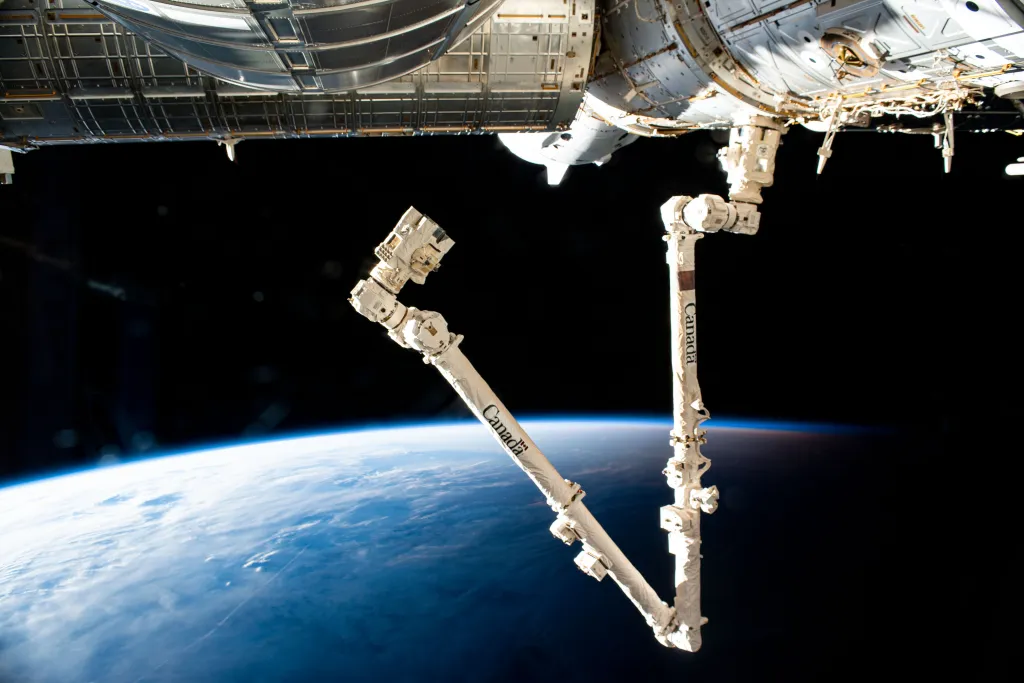
\includegraphics[width=1\linewidth]{1 Introducao/Imagens/Canadarm2.png}
    \caption{Canadarm2 a bordo da ISS. Fonte: NASA.}
    \label{fig:Canadaarm2Foto}
\end{figure}

O \emph{Canadarm2} mede 17,6 metros de comprimento e possui sete juntas que permitem amplo movimento.
Ele pode ser controlado tanto pelos astronautas a bordo da ISS quanto pelos operadores em terra, demonstrando novamente a integração entre a automação e a supervisão humana.

\section{Progress}

A \emph{Progress} é uma espaçonave não-tripulada desenvolvida pela Rússia para missões de reabastecimento à ISS, porém já era utilizada anteriormente às estações espaciais soviéticas, \emph{Salyut} e a \emph{Mir}.
Desde seu primeiro voo em 1978, a \emph{Progress} transportou suprimentos como alimentos, água, oxigênio, equipamentos científicos e combustível.
Além da função de reabastecimento, a \emph{Progress} também é usada para remover resíduos da ISS \cite{progress}.

\begin{figure}[H]
    \centering
    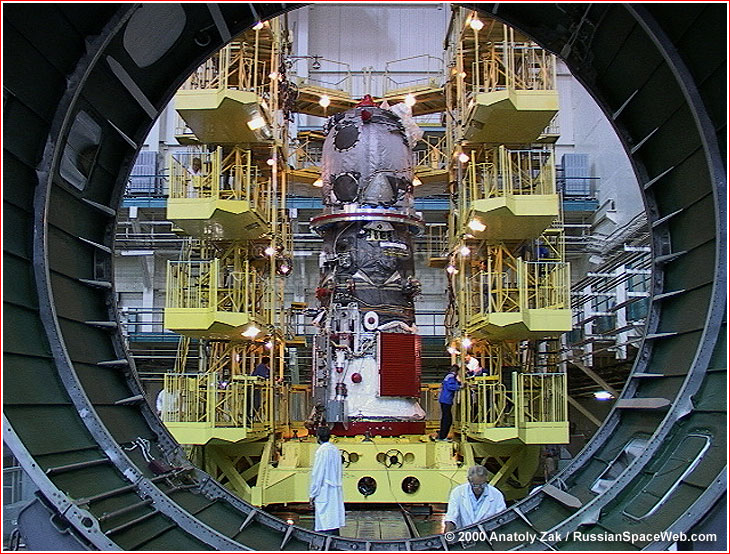
\includegraphics[width=1\linewidth]{1 Introducao/Imagens/Progress.jpg}
    \caption{Espaçonave Progress em construção. Fonte: RussianSpaceWeb.}
    \label{ProgressFoto}
\end{figure}

Embora possua algumas modificações, a espaçonave \emph{Progress} é baseada no design da espaçonave \emph{Soyuz}.
Ela consiste em três módulos principais, sendo um módulo de carga pressurizado, um tanque de combustível não pressurizado e um módulo de propulsão; esse design permite que a \emph{Progress} transporte tanto carga seca quanto líquidos.
Após completar sua missão, a \emph{Progress} é desacoplada para realizar a reentrada na atmosfera terrestre, onde ela é queimanda junto com os resíduos coletados da estação \cite{progress}.
Ao longo das décadas, por conta de sua capacidade de transportar grandes volumes de carga, aliada à sua simplicidade operacional, a tornou uma solução eficiente para o suporte logístico de longo prazo em órbita baixa terrestre (\emph{Low Earth Orbit, LEO}) \cite{progress}.

\section{ATV}

O \emph{Automated Transfer Vehicle} (ATV) foi um veículo de reabastecimento não-tripulado desenvolvido pela Agência Espacial Europeia (ESA) para transportar oxigênio e combustível para ISS.
Seu voo ocorreu pela primeira vez em 2008 e além de possuir um design inovador e altamente automatizado, o ATV também utilizava seus próprios motores para ajustar a órbita da ISS \cite{esaATV}.

Cada missão do ATV era composta por uma espaçonave descartável lançada a partir do foguete \emph{Ariane V}. A espaçoanve era equipado com sistemas automáticos de navegação e de acoplamento para conectar-se à ISS sem a intervenção humana direta.
Após o término da missão, de forma similar a \emph{Progress}, o ATV era desacoplado da estação e direcionado para reentrada controlada na atmosfera terrestre, sendo destruído junto com resíduos descartados da ISS \cite{esaATV}.
Ao longo de suas cinco missões bem-sucedidas entre 2008 e 2015, o ATV contribuiu com tecnologias avançadas para a ISS e serviu como plataforma de testes científicos para estudo de novas tecnologias que poderiam ser aplicadas em futuras missões espaciais como a exploração do espaço profundo \cite{esaATV}.

\section{Acoplamento automático entre duas espaçonaves}

O problema de realizar o acoplamento automático entre duas espaçonaves tem sido historicamente negligenciado devido à disponibilidade de pilotos humanos que assumiam essa função.
Contudo, a União Soviética demonstrou um sistema para acoplamento automático entre dois veículos controlados e ativos, destacando assim, a necessidade de explorar mais esse tipo de missão.
Durante o período em que o estudo foi conduzido, em 1981, ainda não havia sido desenvolvido ou testado em voo um esquema automático de acoplamento em que um dos veículos permanecesse completamente inativo.
Essa lacuna tecnológica evidenciava a necessidade de avançar na capacidade de acoplamento automático, especialmente para aplicações como a recuperação de satélites e a construção de estruturas espaciais.

O trabalho apresentado por \cite{micheal1981} surgiu como parte do projeto \emph{Teleoperator Retrieval System (TRS)}, cuja missão inicial era impulsionar a \emph{Skylab} para uma órbita mais alta, prolongando sua vida útil no espaço. Durante o desenvolvimento do \emph{TRS}, foram analisados os problemas associados ao acoplamento entre o \emph{TRS} e a \emph{Skylab}. 
O estudo abordou um cenário de missão representativo para identificar os requisitos de extração de dados de atitude e posição relativa. Um sistema de acoplamento autônomo foi simulado digitalmente, utilizando dispositivos como sensores de varredura a laser e câmeras de vídeo, que resultou em um desenvolvimento de esquemas automáticos de acoplamento baseados em vídeo poderia representar um avanço significativo em operações de acoplamento em órbita.
Além disso, enfatizou-se a necessidade de maior integração entre sistemas de sensoriamento e algoritmos de controle para reduzir o tempo de treinamento e aumentar a eficiência operacional \cite{micheal1981}.

Por outro lado, o ATV foi um dos maiores contribuidores com a tecnologia de RVD/B, pois a cada missão o veículo realizava uma série de manobras planejadas e ajustava sua posição e velocidade com base em dados em tempo real \cite{esaATVRendezvous}.

\begin{figure}
    \centering
    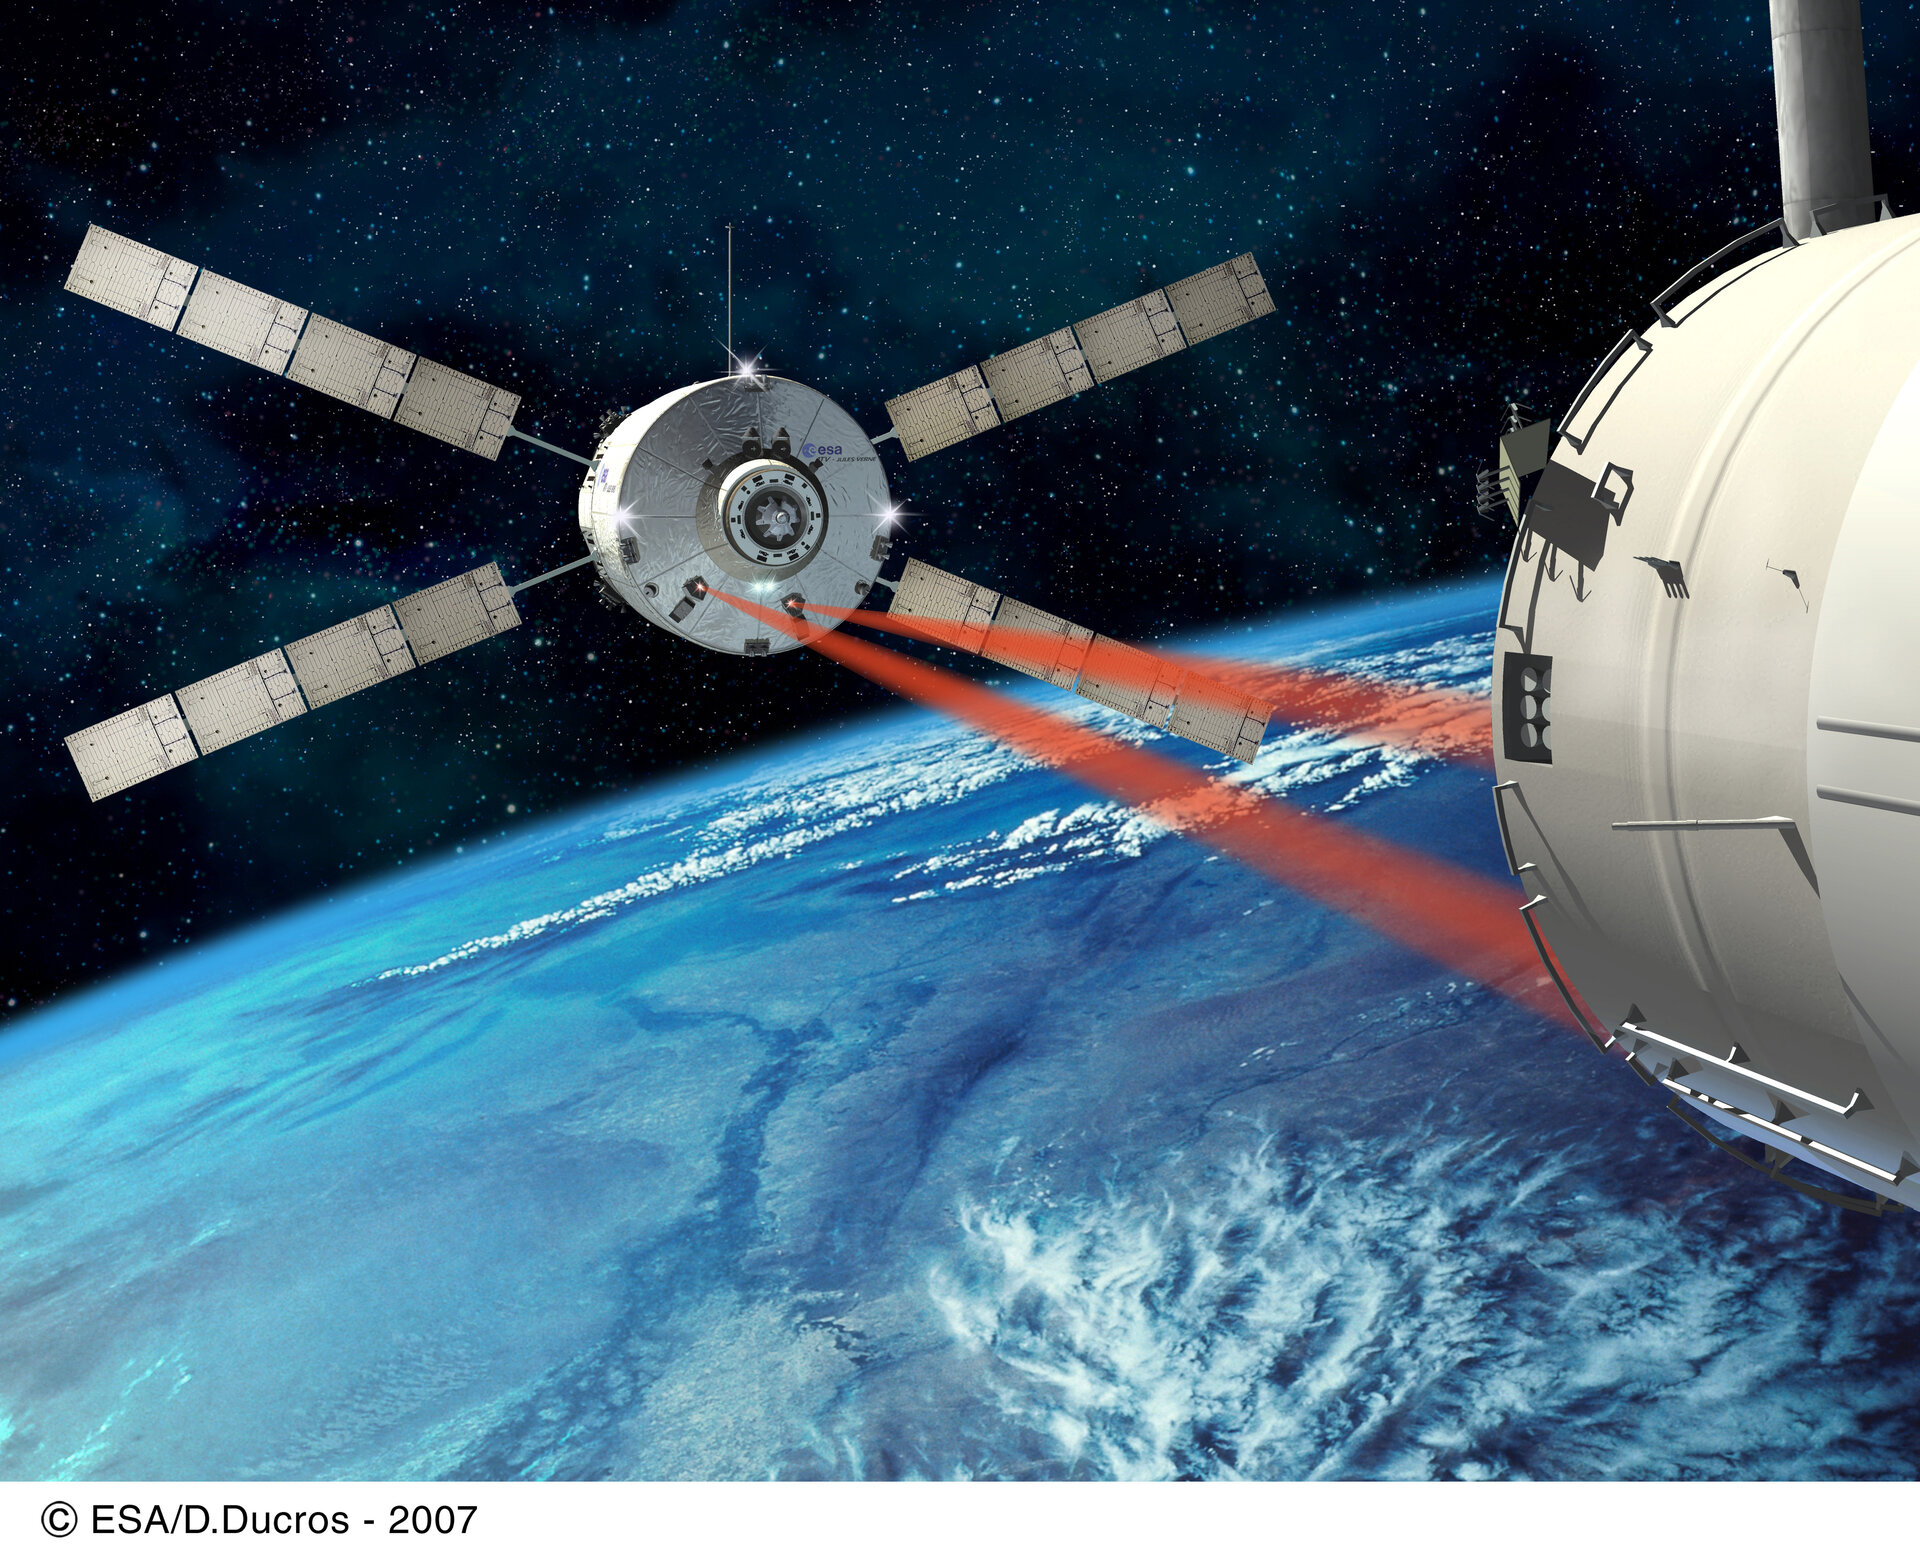
\includegraphics[width=1\linewidth]{1 Introducao/Imagens/ATV RVD.jpg}
    \caption{Simulação da espaçonave ATV realizando rendezvous. Fonte: ESA.}
    \label{fig:ATVAutoDocking}
\end{figure}

O sistema de navegação do ATV integrava sensores, GPS e câmeras, que trabalhavam em conjunto para fornecer informações detalhadas sobre a posição relativa e a orientação da espaçonave em relação à ISS.
Esses dados integrados permitiam ajustes contínuos na trajetória do ATV.
Essa automação completa do processo minimizava a necessidade de intervenção dos operadores a bordo da ISS ou da estação terrestre, o que o tornava confiável e reduzia o risco de erro \cite{esaATVRendezvous}.
Durante a fase final do rendezvous, o ATV utilizava um sistema de guiamento a laser para medir a distância e a orientação em relação à ISS. Além disso, ele ainda contava com algoritmos para garantir que o processo fosse executado com segurança mesmo em cenários de falha parcial de sensores ou de algum outro sistema \cite{esaATVRendezvous}.

Sendo assim, as missões do ATV demonstraram que sistemas de RVD/B totalmente automatizados eram viáveis e eficazes para operações orbitais.
Com isso, abriu-se caminho para o desenvolvimento de tecnologias de navegação e acoplamento, incluindo aquelas destinadas à exploração de espaço profundo, ressaltando o papel da automação na expansão das capacidades humanas no espaço \cite{esaATVRendezvous}.